\documentclass[11pt]{article}
\author{Lawrence Liu}
\usepackage{subcaption}
\usepackage{graphicx}
\usepackage{amsmath,amssymb,stmaryrd}
\usepackage{physics}
\usepackage{pdfpages}
\newcommand{\Laplace}{\mathscr{L}}
\setlength{\parskip}{\baselineskip}%
\setlength{\parindent}{0pt}%
\usepackage{xcolor}
\usepackage{listings}
\definecolor{backcolour}{rgb}{0.95,0.95,0.92}
\usepackage{amssymb}
\lstdefinestyle{mystyle}{
    backgroundcolor=\color{backcolour}}
\lstset{style=mystyle}
\title{Physics 115C HW 3}
\begin{document}
\maketitle
\section*{Problem 1}
\subsection*{(a)}
Since the ground state should have no nodes, we would expect it to be 
symmetric. And since the first excited state should have 
be orthogonal to the ground state, we would expect it to be antisymmetric.
Therefore a rough sketch of the wavefunctions would be:
% \begin{figure}[h]
%     \centering
    \\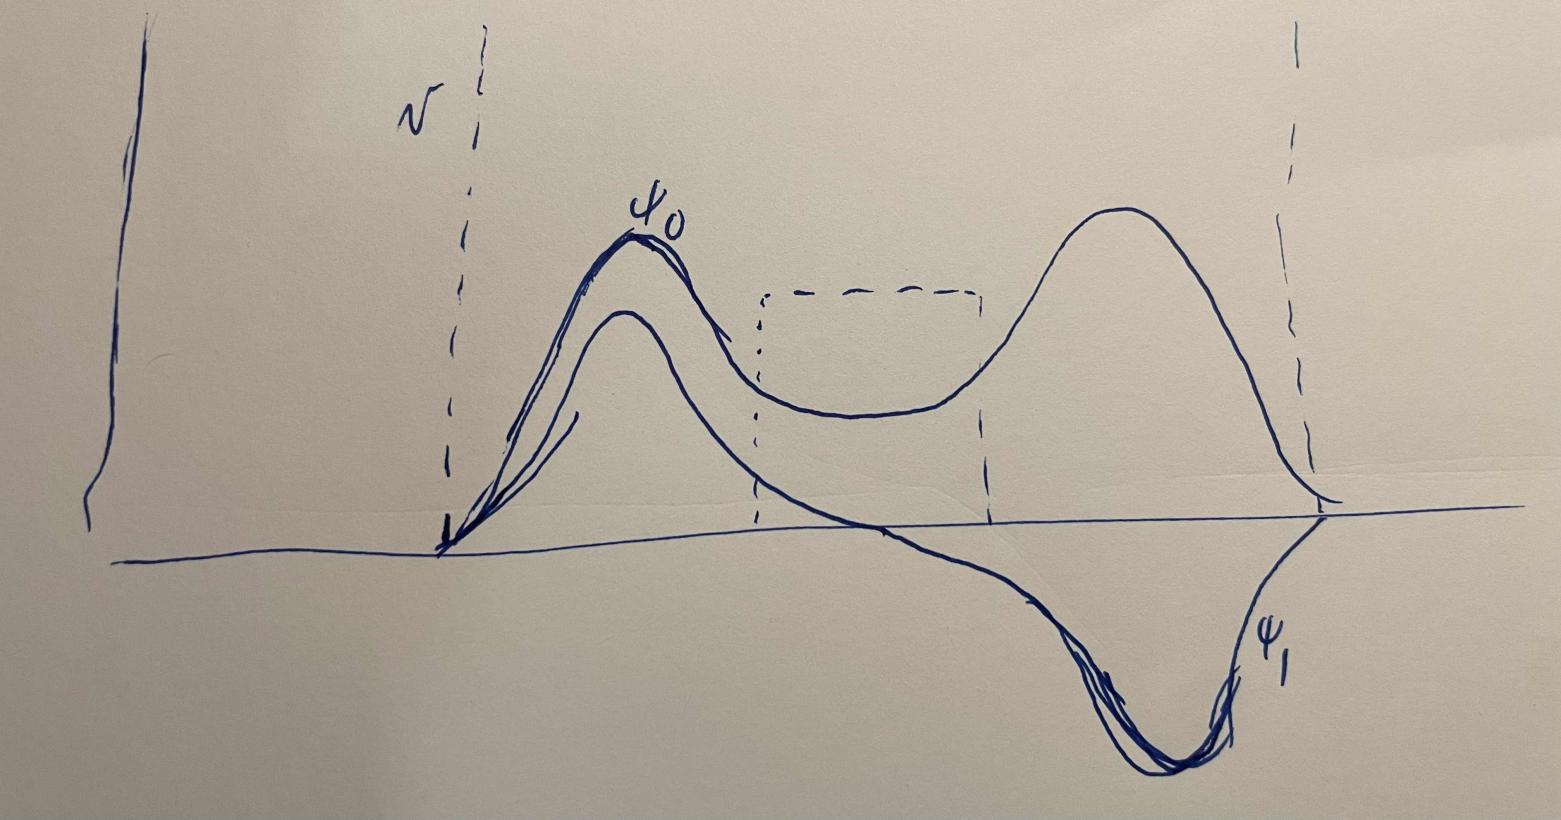
\includegraphics[width=0.5\textwidth]{prob1a.png}
%     \caption{Sketch of the ground state and first excited state wavefunctions}
% \end{figure}
\subsection*{(b)}
We have that if the central barrier height is $0$, then the problem becomes the 
infinite square well problem. Therefore the ground state and first excited state
are:
\\\includegraphics*[width=0.5\textwidth]{prob1b1.png}\\
And if the central barrier height is $\infty$, then the particle cannot exist in the 
center. Therefore the ground state and first excited state are:
\\\includegraphics*[width=0.5\textwidth]{prob1b2.png}\\
Thus we can see that the splitting will be large when the central barrier is close to $0$, and 
large when the central barrier is close to $\infty$.
\subsection*{(c)}
\includegraphics*[width=0.5\textwidth]{prob1c.png}
\subsection*{(d)}
The $\psi_{\pm}(x)$ wavefunctions are not parity symmetric. However the Hamilonian is 
parity symmetric.
\subsection*{(e)}
The expectation value of $\bra{\psi_{+}}x\ket{\psi_{+}}$ and 
$\bra{\psi_{-}}x\ket{\psi_{-}}$ are bot not $0$ since $\psi_{\pm}(x)$ is 
not parity symmetric. However the expectation value of $
\bra{\psi_{0}}x\ket{\psi_{0}}$ and $\bra{\psi_{1}}x\ket{\psi_{1}}$ are $0$ since 
$\psi_{0}(x)$ and $\psi_{1}(x)$ are parity symmetric.
\subsection*{(f)}
No in the case of finite barrier height we will have that $\ket{\psi_0}$ 
and $\ket{\psi_1}$ will no longer be degenerate. Therefore they will evolve at 
different rates, and thus $\ket{\pm}$ will no longer be stationary states.
\subsection*{(g)}
$$\ket{+(t)} = \frac{1}{\sqrt{2}}\left(
    e^{-iE_0t/\hbar}\ket{0} + e^{-iE_1t/\hbar}\ket{1}
\right)$$
\subsection*{(h)}
The probability that the particle is in state $\ket{-}$ is given by 
\begin{align*}
    |\bra{-}\ket{+(t)}|^2 &= \frac{1}{4}\left|
        e^{-iE_0t/\hbar} + e^{-iE_1t/\hbar}\right|^2\\
        &= \frac{1}{4}\left(
            (\cos(\frac{E_0t}{\hbar}) + \cos(\frac{E_1t}{\hbar}))^2 + 
            (\sin(\frac{E_0t}{\hbar}) + \sin(\frac{E_1t}{\hbar}))^2
        \right)\\
        &= \frac{1}{4}\left(
            2 + 2\cos(\frac{(E_0 - E_1)t}{\hbar})\right)
\end{align*}
Therefore we can see that the first time particle will turn 
into state $\ket{-}$ is when $t = \frac{\pi\hbar}{E_1 - E_0}$.
\subsection*{(i)}
As we raise the barrier height, the splitting between the ground state and 
the first excited state will decrease therefore 
the time it takes for the particle to turn into state $\ket{-}$ will increase. And when 
the barrier height becomes infinite, the particle will never turn into state $\ket{-}$. 
\subsection*{(j)}
$$\frac{2\pi\hbar}{E_1-E_0} = \frac{1}{24\cdot10^9}$$
$$E_1-E_0 = 1.590\cdot 10^{-23}J$$
The wavelength of the light emited is given by 
$$\lambda = \frac{hc}{E_1-E_0} = 0.012m$$
Therefore we can see that the wavelength of the light emited is in the
microwave range. 
\subsection*{(k)}
The time it would take to tunnel is 
$$\frac{1}{2\cdot 160\mu \text{Hz}} = 3125s$$
This tunneling time is much longer than Ammonia, therefore we can conclude 
that the barrier height for $AsH_3$ is much higher than that of Ammonia.
\subsection*{(l)}
It would depend how long the measurement is taken. Both atoms have an "instantenous" dipole,
ie if we measure instantenously, we will find that the dipole is non-zero, since the 
As or N atom will be on one side of hydrogen plane. But when
the As or N atom oscillates to the other side of the hydrogen plane, the dipole will flip.
So the net dipole if we measure for a long time (on the order of days) will be $0$.
\section*{Problem 2}
\subsection*{(a)}
From the periodic boundary condition we must have that:
$$\psi(x) = \psi(x+L)$$
$$Ne^{ikx} = Ne^{ik(x+L)}$$
$$e^{ikL} = 1$$
$$kL = 2\pi n$$
$$\hbar k = \frac{2\pi \hbar n}{L}$$
\subsection*{(b)}
We must have that
$$\int_{-\infty}^{\infty}|\psi(x)|^2dx = 1$$
$$\int_{0}^{L}|\psi(x)|^2dx = 1$$
$$\int_{0}^{L}N^2dx = 1$$
$$N = \frac{1}{\sqrt{L}}$$
\subsection*{(c)}
The energy eigenvalues are 
$$E_n = \frac{\hbar^2k^2}{2m} = \frac{\hbar^2(2\pi n)^2}{2mL^2}$$
Therefore we can see that the $+n$ and $-n$ energy eigenvalues are the same, 
and thus are degenerate.
\subsection*{(d)}
The perturbation can be written as 
$$H' = -\beta p$$
$$H' = -\beta \frac{\hbar}{i}\frac{d}{dx}$$
We can see that this commutes with the hamiltonian, $H=\frac{1}{2m}p^2$.
Therefore the eigenstates we would use would be the energy eigenstates of the 
original unperturbed hamiltonian.
\subsection*{(e)}
We have that the first order correction to the energy is given by
$$E_{n}^1 = \bra{n}H'\ket{n}$$
$$E_{n}^1 = -\beta \bra{n}\frac{\hbar}{i}\frac{d}{dx}\ket{n}$$
$$E_{n}^1 = -\beta \frac{\hbar}{i}\int_{0}^{L}\psi_n^*(x)\frac{d}{dx}\psi_n(x)dx$$
$$E_{n}^1 = -\beta \frac{\hbar}{L}k_n$$
$$E_{n}^1 = \boxed{-\beta \frac{2 \pi \hbar n}{L}}$$
\subsection*{(f)}
\includegraphics*[scale=0.5]{2f.png}
As we can see the lifting of degeneracy does not affect each pair in the same way, 
the higher $n$ states have a larger energy shift than the lower $n$ states.
\subsection*{(g)}
Yes there is a degeneracy in the system, when 
$\beta_z = \frac{2\pi\hbar z}{2mL}$ the $z$th excited state will 
be degenerate with the unperturbed ground state.
\subsection*{(h)}
No because the perturbation is too big, so we 
cannot use perturbation theory.
\subsection*{(i)}
Yes because the perturbation has the same eigenstates to 
the unperturbed hamiltonian, therefore we would have that the 
new energy eigenvalues $E_n$ would just be given by 
$$E_{n} = \bra{n}H+H'\ket{n}$$
$$E_{n} = \bra{n}H\ket{n} + \bra{n}H'\ket{n}$$
THerefore we can see the correction to the energy eigenvalue:
$$E_{n}-\bra{n}H\ket{n} = \bra{n}H'\ket{n}$$
Which is the same value we derived with 
perturbation theory.
\subsection*{(j)}
We have that:
$$\ket{\psi_n^{1}}= \sum_{m\neq n}\frac{\bra{m}H'\ket{n}}{E_n-E_m}\ket{m}$$
Since $\ket{n}$ for all $n$ are eigenstates of $H'$, we have that 
$\bra{m}H'\ket{n} = 0$ for all $m\neq n$. Therefore we have that
$$\ket{\psi_n^{1}}= 0$$
Which is what we expected from the fact that the perturbation commutes 
with the hamiltonian.
\subsection*{(k)}
We have that the second order correction to the energy is given by
$$E_{n}^2 = \sum_{m\neq n}\frac{|\bra{m}H'\ket{n}|^2}{E_n-E_m}$$
As we noted before $\bra{m}H'\ket{n} = 0$ for all $m\neq n$. Therefore we have that
$$E_{n}^2 = 0$$
This is what we expected from the fact that the perturbation commutes with the hamiltonian
and thus how the energy correction from first order perturbation theory is the exactly
what the energy correction is when we calculate the energy eigenvalue directly. Likewise, 
we would expect the higher order corrections to be $0$ as well for the same reason.
\section*{Problem 3}
\subsection*{(a)}
We have that 
\begin{align*}
    \bra{1}H'\ket{1}&=\frac{1}{L}\int_{0}^{L}V\sin\left(\frac{4\pi x}{L}\right)dx\\
    &=0
\end{align*}
Likewise 
\begin{align*}
    \bra{-1}H'\ket{-1}&=\frac{1}{L}\int_{0}^{L}V\sin\left(\frac{4\pi x}{L}\right)dx\\
    &=0
\end{align*}
We also have that 
\begin{align*}
    \bra{1}H'\ket{-1}&=\frac{1}{L}\int_{0}^{L}e^{-ik_1x}V\sin\left(\frac{4\pi x}{L}\right)e^{-ik_1x}dx\\
    &=\frac{V}{2Li}\int_{0}^{L}(e^{\frac{i4\pi x}{L}}-e^{-\frac{i4\pi x}{L}})e^{-i\frac{4\pi}{L}x}dx\\
    &=\frac{V}{2Li}\int_{0}^{L}(1-e^{-\frac{i8\pi x}{L}})dx\\
    &=\frac{V}{2Li}\left.\left(x+\frac{L}{8i\pi}e^{-\frac{i8\pi x}{L}}\right)\right|_{0}^{L}\\
    &=\frac{V}{2Li}\left(L+\frac{L}{8i\pi}-\frac{L}{8i\pi}\right)\\
    &=\frac{V}{2i}\\
\end{align*}
Likewise we have that
\begin{align*}
    \bra{-1}H'\ket{1}&=\frac{1}{L}\int_{0}^{L}e^{ik_1x}V\sin\left(\frac{4\pi x}{L}\right)e^{ik_1x}dx\\
    &=\frac{V}{2Li}\int_{0}^{L}(e^{\frac{i4\pi x}{L}}-e^{-\frac{i4\pi x}{L}})e^{i\frac{4\pi}{L}x}dx\\
    &=\frac{V}{2Li}\int_{0}^{L}(e^{\frac{i8\pi x}{L}}-1)dx\\
    &=\frac{V}{2Li}\left.\left(\frac{L}{8i\pi}e^{\frac{i8\pi x}{L}}-x\right)\right|_{0}^{L}\\
    &=-\frac{V}{2i}\\
\end{align*}
Therefore we have that
$$\begin{bmatrix}
    0 & \frac{V}{2i}\\
    -\frac{V}{2i} & 0
\end{bmatrix}=\frac{V}{2i}\begin{bmatrix}
    0 & 1\\
    -1 & 0
\end{bmatrix}$$
The eigenvalues of $\begin{bmatrix}
    0 & 1\\
    -1 & 0
\end{bmatrix}$ are $\pm i$. Therefore we have that the first order 
correction to the energy is $\pm \frac{V}{2}$.
\subsection*{(b)}
The eigenvectors of the matrix $\begin{bmatrix}
    0 & 1\\
    -1 & 0
\end{bmatrix}$ are $\begin{bmatrix} -i \\ 1 \end{bmatrix}$ and $\begin{bmatrix} i \\ 1 \end{bmatrix}$.
Therefore we have that the normalized good states are:
$$\frac{1}{\sqrt{2}}(\ket{-1}\pm i\ket{1})$$
\subsection*{(c)}
Because $\bra{2}\ket{2}=\bra{-2}\ket{-2}=1$ we still have that 
$$\bra{2}H'\ket{2}=\bra{-2}H'\ket{-2}=0$$
However we have that
\begin{align*}
    \bra{-2}H'\ket{2}&=\frac{1}{L}\int_{0}^{L}e^{ik_2x}V\sin\left(\frac{4\pi x}{L}\right)e^{-ik_2x}dx\\
    &=\frac{V}{2Li}\int_{0}^{L}(e^{\frac{i4\pi x}{L}}-e^{-\frac{i4\pi x}{L}})e^{-i\frac{8\pi}{L}x}dx\\
    &=0
\end{align*}
And since $(\bra{-2}H'\ket{2})^*=\bra{2}H'\ket{-2}$ we have that $\bra{2}H'\ket{-2}=0$ as well.
Therefore we have that the first order shift to the second lowest 
energy level is $0$.
\subsection*{(d)}
The energy split by $V$ for the lowest energy degenerate state and $0$ for 
second highest energy degenerate state.
\subsection*{(e)}
The highest energy degenerate states should not be lifted as well, since the 
we would have that 
$$\bra{-n}H'\ket{n} = \frac{V}{2iL}\int_{0}^{L}e^{i2k_nx}(e^{i4\pi x/L}-e^{-i4\pi x/L})dx = 0$$
if $n>1$ then we will have that this integral becomes the integral of 
$$e^{i\pi \frac{x}{L}(4-2n)} - e^{i\pi \frac{x}{L}(-4-2n)}$$
Which for $n>1$ is periodic with $L$ and thus the integral is $0$. And as we noted before
since $(\bra{-n}H'\ket{n})^*=\bra{n}H'\ket{-n}$ we have that $\bra{n}H'\ket{-n}=0$ as well. And 
we will have that $\bra{-n}H'\ket{-n}=\bra{n}H'\ket{n}=0$ as well. Therefore we have that the 
first order correction to the energy is $0$ for all $n$.
\subsection*{(f)}
If we changed the wavelength of the perturbation to $\lambda = \frac{L}{2^n}$ then we would split the 
$n$ degenerate state instead.








\end{document}
 
